\documentclass[conference]{IEEEtran}

\usepackage[utf8]{inputenc}
\usepackage[T1]{fontenc}
\usepackage{silence}\WarningsOff[latexfont]

\usepackage{amsmath}
\usepackage{nicefrac}

\usepackage{graphicx}
\usepackage{cite}
\usepackage{url}
\usepackage[caption=false,font=footnotesize]{subfig}
\usepackage[binary-units,per-mode=symbol]{siunitx}
\sisetup{list-final-separator = {, and }}
\usepackage{booktabs}
\usepackage{pifont}
\usepackage{microtype}
\usepackage{textcomp}
\usepackage[american]{babel}
\usepackage[noabbrev,capitalise]{cleveref}
\usepackage{xspace}
\usepackage{hyphenat}
\usepackage[draft,inline,nomargin,index]{fixme}
\fxsetup{theme=color}
\usepackage{grffile}
\usepackage{xfrac}
\usepackage{multirow}
\RequirePackage{xstring}
\RequirePackage{xparse}
\RequirePackage[index=true]{acro}
\NewDocumentCommand\acrodef{mO{#1}mG{}}{\DeclareAcronym{#1}{short={#2}, long={#3}, #4}}
\NewDocumentCommand\acused{m}{\acuse{#1}}
\usepackage{upquote}

\begin{document}

\title{
	A Gossip-Style Failure Detection Service \\
    \large Distributed Systems 2 - Final Project - University of Trento
}

\author{
	\IEEEauthorblockN{Andrea Zorzi}
	\IEEEauthorblockA{\small Matriculation number: 190964 \\ andrea.zorzi-1@studenti.unitn.it}
    \and
    \IEEEauthorblockN{Davide Vecchia}
    \IEEEauthorblockA{\small Matriculation number: 188776 \\ davide.vecchia@studenti.unitn.it}
    \and
    \IEEEauthorblockN{Davide Pedranz}
    \IEEEauthorblockA{\small Matriculation number: 189295 \\ davide.pedranz@studenti.unitn.it}
}

\maketitle

\begin{abstract}
Failure detection allows to solve traditionally difficult problems in distributed systems,
such as reliable broadcast and consensus.
In this work, we implement and test a gossip based failure detection service.
We describe the basic protocol on which this work is based and some variants;
then, we describe how we experimentally tested and tuned the systems;
finally, we analyse the obtained results and give suggestions on how to choose the best parameters based on the needed performances of the failure detector for real-world systems.
\end{abstract}

\acresetall

\section{Introduction}
\label{sec:introduction}

A failure detector can be described as a distributed oracle that provides information about the state of the other processes in the system.
From a practical point of view, it is a service that detects when the other processes are not available, for instance when they crash or become not reachable.
Failure detectors can be used to solve difficult problems in distributed systems, such as reliable broadcast, consensus and group membership.

A simple way to build a failure detector is to periodically ping each other process.
On the one hand, the idea is effective and easy to implement; on the other hand, the resulting protocol is very inefficient, since it produces $O(n^2)$ messages every ``round'' (where $n$ is the number of the processes).
For extreme distributed systems, this approach does not scale.

An alternative approach to build failure detectors is to use gossip.
In gossip-based protocols, processes exchange information with random peers at regular intervals.
In our case, they exchange information about the processes which are still gossiping:
if a process does not gossip anymore, it is probably crashed or unreachable.
This approach was firstly proposed by Van Renesse, Minsky and Hayden in 1998 in the paper ``A Gossip-Style Failure Detection Service'' \cite{gsfd}.
The authors describe a protocol based on gossip to provide timely and efficient failure detection and provide a backup protocol based on broadcast to recover from catastrophes (for example, when half of the nodes crashes at the same time).

In this work, we implement and test a protocol based on the original paper.
We try some modifications to the original proposal and measure their effect.
We also tune the performances to match the computing power and network capabilities of modern distributed systems.

\cref{sec:paper} describes in detail the original work.
\cref{sec:variants} shows some little modifications to improve the protocol.
\cref{sec:implementation} describes how we implement the protocol.
\cref{sec:metrics} shows how we evaluate and test the protocol.
Finally, \cref{sec:experiments} discuss which modifications help the original protocol and which do not.
To conclude, we describe a simple yet effective way to tune the performances based on real world needs.

\section{Original Work}
\label{sec:paper}

The protocol presented in the paper is able to detect failures with some specified probability of mistake (false positive),
with the valuable property that the detection time scales as \nobreak{$O(n\nobreak\hspace{.08em}\cdot\nobreak\hspace{.08em}log(n))$} with respect to the number of nodes.
The protocol is not able to discriminate between a crashed node from a slow or unreachable one (e.g. communication failures):
a detection is interpreted as a general ``the node is not available''.
Each node has a ``heartbeat'' counter which is incremented at each round of gossip.
Periodically, each node exchanges its own and the others counters with a random peer.
If a node does not hear any heartbeat update for some node for a given time, it assumes it has crashed.

At the beginning of the protocol, each node activates a timer $T_{gossip}$.
Upon timeout, it increments its own heartbeat counter.
Then, it randomly selects another node to infect and sends the most recent heartbeat counter it knows for each member.
Finally, the timer is restarted.

For each node of the system, a timer $T_{fail}$ is set and the countdown is started.
Upon timeout, the relative node is considered failed.
$T_{fail}$ is chosen so that there is a really low probability that any node's timeout triggers before the ``infection'' (the update on a heartbeat counter) arrives to all members.

When a node receives a gossip message with current heartbeat counters of the sender,
it updates those counters it stores locally that are lower than the received ones.
If a heartbeat counter is updated, the timer associated to that node is reset to $T_{fail}$.

With some modification, the protocol can resist a ``catastrophe'', i.e. when many nodes become simultaneously unavailable (for example due to a network failure that separates groups of nodes).
In case of a catastrophe, some additional time is required to prevent correct nodes from reporting each other as failed.
This happens because a portion of messages is wasted gossiping with unavailable nodes, so the protocol between correct nodes not only has a virtually increased gossip interval, but also has a slower progression because messages towards those unavailable nodes do not contribute to progress.
Information on heartbeat counters has not enough time to infect the whole network, causing those false positives.
Together with the extra time, a multicast protocol is enabled.
With some probability that grows over time, nodes will send a special message to all the others and wait for a reply to obtain the most up-to-date heartbeat counters.
If tuned correctly, this parameter ensures that one surviving node will be able to gossip an information that will keep nodes of the correct portion from reporting each other, making the recovery more reliable. 

If catastrophe recovery is enabled, a node is not immediately reported after $T_{fail}$, but during the additional time it can not be chosen to be a gossip recipient (restoring the natural gossip interval of the system as well as the statistical guarantees for progression).
Eventually, all correct nodes will hear updates of each other and restart the $T_{fail}$ timer.

Once a node marks another one as failed, it waits a time $T_{cleanup} = 2 \cdot T_{fail}$ before removing its association with the heartbeat counter in the gossiped list.
This is done to prevent the reappearance of a failed node.
Consider a node F reported as failed and undergoing cleanup.
Of course, the heartbeat counter of F can not be updated.
It is safe to wait $2 \cdot T_{fail}$ before removing F:
after $T_{fail}$ every process is infected by updates on F that may be still circulating, and then after another $T_{fail}$ - since there is no new circulating infection - every node considers F failed and thus will not update its heartbeat counter.

\section{Variants}
\label{sec:variants}

We propose two different variants to the original protocol.
The first one is related to the way the nodes gossip with each other.
The second one is about how nodes chooses their peers.
We discuss the effect of these changes in \cref{sec:experiments}.


\subsection{Push-Pull}
The protocol described in the original paper uses the Pull approach.
In other words, a node selects its peer and sends it a message with some information.
The peer receives the message but does not reply.

The Push-Pull approach introduces an additional step.
The selected peer receives the message, updates its local knowledge about the systems and replies to the sender with its up-to-date information.
The sender receives the reply and updates its own one.
The idea behind Push-Pull is to spread the information as fast as possible.


\subsection{Peer Selection Strategy}
In the basic protocol, each node selects its peer randomly at each round of gossip.
We propose some different peer selection strategies that try to exploit the local knowledge to make a better choice.

\paragraph*{Quiescence}
The probability to select a node is linear with respect to its quiescence, i.e. the difference (in gossip intervals) between the current time and the last heartbeat update received for that node.

\paragraph*{Squared Quiescence}
The probability to select a node is proportional to the square of its quiescence.

\paragraph*{Highest Quiescence}
Always select the node with the oldest update.
If more than one node share the oldest update time, select one randomly.

\section{Implementation}
\label{sec:implementation}

The implementation is based on the description of the original paper.
We make some simplifying assumptions so that testing the protocol is simpler, but do not alter the core concepts of the algorithm.

\subsection{Assumptions}

We make the following assumptions about the system:
\begin{itemize}
    \item asynchronous system (no strict bounds on message delivery time, we just assume the network operates reasonably)
    \item nodes know each other
    \item nodes can not join or leave the system during an experiment run
    \item fail-stop failure model (no Byzantine behaviour is allowed)
\end{itemize}

The protocol is implemented using Akka\footnote{\url{http://akka.io/}}, a framework for the Java Virtual Machine to build distributed systems based on the actor pattern.
Akka provides a simple API to create actors and asynchronously send messages between them.
The framework hides the network communication and takes care to build and maintain the overlay network between the actors.

\subsection{Tracker}
The tracker actor has the role to run the experiments needed to test the gossip protocol.
It tracks the nodes of the system, runs the experiments, collects the failures detected by each node and generates a report with the results for further offline elaboration.

The tracker runs on a dedicated machine with a public IP address known to all nodes.
When a new node is started, it registers immediately to the tracker and waits for instructions.
Depending on its configuration, the tracker waits until a certain number of nodes join the system.
Once the number is reached, the tracker generates a list of experiments to perform.

The experiments are run one at a time, in a sequential order.
Upon an experiment start, the tracker sends a start message to each node:
the start message contains the list of nodes running the current experiment and the parameters to use for the gossip protocol.
Since it is unrealistic that a node crashes during an experiment, node failures are simulated.
The tracker schedules a list of failures and instruct the nodes to crash at some fixed delta of time after the start of the experiment.
Nodes asked to simulate a failure simply stop to send or reply to any message coming from other nodes (with the exception of the tracker).
Every time a node detects a failure, it reports it to the tracker.

At the end of the experiment (i.e. after some fixed time), the tracker send a stop message to all nodes.
Before starting the next experiment, the tracker generates a report with the settings of the experiment, the scheduled crashes and the reported ones.
The report is exported as a \texttt{JSON} file and stored on the disk.
At this point, the tracker waits some time to make sure all nodes received the stop message, then starts the new experiment.
When the nodes receive a stop message, they stop to gossip with each other and reset the internal state: they are ready for the next experiment.


\subsection{Node}
The node actor implements the gossip-based failure detector.

If asked by the tracker at the start of an experiment, a node schedules a crash simulation to happen at the specified time.

Each node keeps a structure with all nodes in the system and their relative heartbeat counters.
This is the information exchanged in the gossip protocol.
Another structure contains those nodes that are considered correct:
their heartbeat counters can be updated and they can be selected as gossip recipient.

If the backup protocol to resist to catastrophes is enabled, nodes that may be still correct but whose state is currently unknown are saved in a disjoint subset, and are considered ``missing''.
A node that is missing cannot be selected as a gossip recipient.
However, if a message is received that would increment the heartbeat counter of a missing node, that node is restored as correct.
Practically, once $T_{fail}$ is exhausted, an additional timer $T_{miss}$ is started.
After $T_{miss}$, except if the node was restored as correct, it is reported to the tracker as failed.
The multicast protocol is configured so that nodes wait at most a time equal to $T_{fail}$ to multicast, and generally it happens at around $T_{fail}/2$.
A node decides whether to multicast or not every second, and the probability increases each time it is postponed, until either the attempt is successful or it receives a multicast message from another node.
Once a node receives the special message, it sends back its structure with heartbeats.
The purpose of the protocol is to help spreading updated information.
The maximum wait for multicast is set to be equal to $T_{fail}$ in order to have that information readily available after the catastrophe, after $T_{fail}$ in the worst case.
Assuming this, $T_{miss}$ can more easily be decided.

The structure with all nodes of the system may contain some that is neither missing nor correct.
Those are considered failed.
They will be finally removed only after $T_{cleanup}$.

A node may reappear at some nodes if its heartbeat counter is still circulating in the network inside gossip messages after $T_{cleanup}$.
Since we assume each node always has knowledge of all the others, waiting $T_{cleanup}$ would be unnecessary:
a node can simply ignore the heartbeat counter associated to a node it considers failed, since it can just decide to never restore a node.
If instead the system could change and possibly grow, a cleanup mechanism would be required.
It is implemented to confirm the soundness of setting $T_{cleanup}$ to $2 \cdot T_{fail}$.

All timers described are implemented as scheduled messages from a node to itself.
These messages can be cancelled before they are sent.
For example, a ``fail'' message is scheduled to happen after $T_{fail}$.
When the heartbeat counter of the relative node is updated, that incoming message is cancelled and a new one is scheduled. Each message has an incremental ID, so that those that should have been cancelled can be recognized and behaviour can be kept consistent even when more messages are enqueued in the node's mailbox.


\subsection{Remote machines}

To perform the experiments, the system (tracker and nodes) has been deployed and ran multiple times on different EC2 machines spread around the world (America, Europe, Asia) on the AWS Cloud\footnote{\url{https://aws.amazon.com/ec2/}}.
A simple command line script to start, stop and manage the experiments has been developed.
For each experiment, the CLI allows us to automatically create one instance of an EC2 machine for each node, deploy our project on the machines, configure the parameters of the experiment and start it in a quick way.
Moreover, the script allows us to keep watching the status of the experiments while they are running, to download the results from the tracker machine once they are finished and shutdown the system.

\section{Evaluation Metrics}
\label{sec:metrics}

Our aim is to build a perfect failure detector.
A perfect failure detector has 2 properties: strong completeness (every crashed process is eventually reported to the tracker) and strong accuracy (no false positives are reported).

An experiment is considered unsuccessful if any of these circumstances occur:
\begin{itemize}
    \item a faulty node is not reported by all correct nodes
    \item a faulty node is reported before the expected crash happens
    \item there are reappearance reports
    \item there are duplicated crash reports
\end{itemize}

We measure the average detection time, expecting it to grow similarly to $T_{fail}$.
The first detection time will be not much greater than $T_{fail}$.
With catastrophe recovery, we cannot have a correct report earlier than $T_{fail} + T_{miss}$ after the crash.
In general, we expect the maximum delay for detection to never exceed $2 \cdot T_{fail}$, or $2 \cdot (T_{fail} + T_{miss})$ with catastrophe recovery.
Clearly, the actual value depends on the required time needed to spread the information. 

\section{Experiments}
\label{sec:experiments}

This section describes the experiments carried out to test our implementation of the failure detection algorithm and what we analyse in order to find the best parameters to use with the algorithm.

Apart from some experiments regarding Push and Push-Pull strategy comparison, all the experiments are performed using a $T_{gossip}$ value of $200 \si{ms}$.

In every experiment (except experiments related to catastrophic scenarios) a single node simulates a crash after a certain period of time and the other nodes have to detect it.

All experiments have a duration of 2 minutes and are repeated using the Push and the Push-Pull gossip strategy.

The first experiments have the aim to understand how the failure detector behaves using different values of  $T_{fail}$ and to discover in which conditions the algorithm performs better.
For this experiments, we use 10, 30 and 50 nodes respectively and different strategies to choose the node to which gossip to.
In the following experiments we decide to use only 50 nodes since we notice that the algorithm scales well (the number of involved nodes does not significantly influence the results).

Next, we focus our attention on how the algorithm behaves in catastrophic conditions.
We run the algorithm simulating a catastrophic event: after a certain period of time, \nicefrac{2}{3} of the nodes belonging to the system crash at the same time.
We perform some experiments to observe how the gossip algorithm behaves in these conditions in combination with the multicast backup protocol.
We also use these experiments to empirically find out a proper value for the $T_{miss}$ parameter.

Finally, some experiments are carried out to understand how the use of different $T_{gossip}$ values for different gossip strategies could influence the failure detection algorithm.


\subsection*{Behaviour with respect to $T_{fail}$}

\begin{figure}[t]
	\centering
	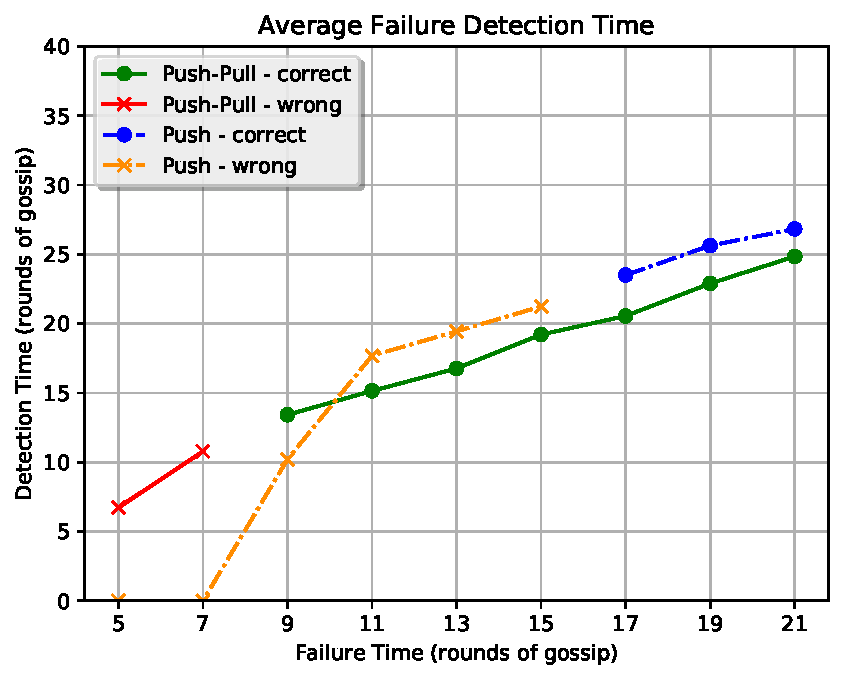
\includegraphics[width=\columnwidth]{figures/n50__average__s0__no_catastrophe__no_multicast}
	\caption{The plot shows the performances of the protocol in case crash of a single out of $50$ nodes. The multicast backup protocol in not enabled. Nodes choose their peers randomly (original strategy) and gossip every $200 \si{ms}$. The Push-Pull variant seems to have better performances for the same values of $T_{fail}$.}
	\label{fig:n50__average__s0__no_catastrophe__no_multicast}
\end{figure}

\cref{fig:n50__average__s0__no_catastrophe__no_multicast} shows correctness and average detection time with varying $T_{fail}$, expressed in terms of gossip intervals.
These experiments clearly show that $T_{fail}$ values under a certain threshold are not suitable.
Since the algorithm is highly probabilistic, even high values of $T_{fail}$ may cause a false detection; in practice, this never happens.
The experiments employing the Push-Pull variant start to behave correctly at a $T_{fail}$ that is roughly half of the one required by Push.
Additionally, average detection time is slightly lower.

High detection times are caused by heartbeat updates that are still circulating in the network after the node crashed.
Since the information spreads faster with Push-Pull, the last node is infected earlier and consequently the detection time lowers.
Some experiments with low $T_{fail}$ are shown with average detection time of 0: this means that there is not even a single correct detection.
There is not enough time for the Push version to gossip with the whole network: nodes start to report each other as crashed.
Even though the actually crashed node is reported, this happened before the actual crash time.


\subsection*{Catastrophe}

\begin{figure}[t]
	\centering
	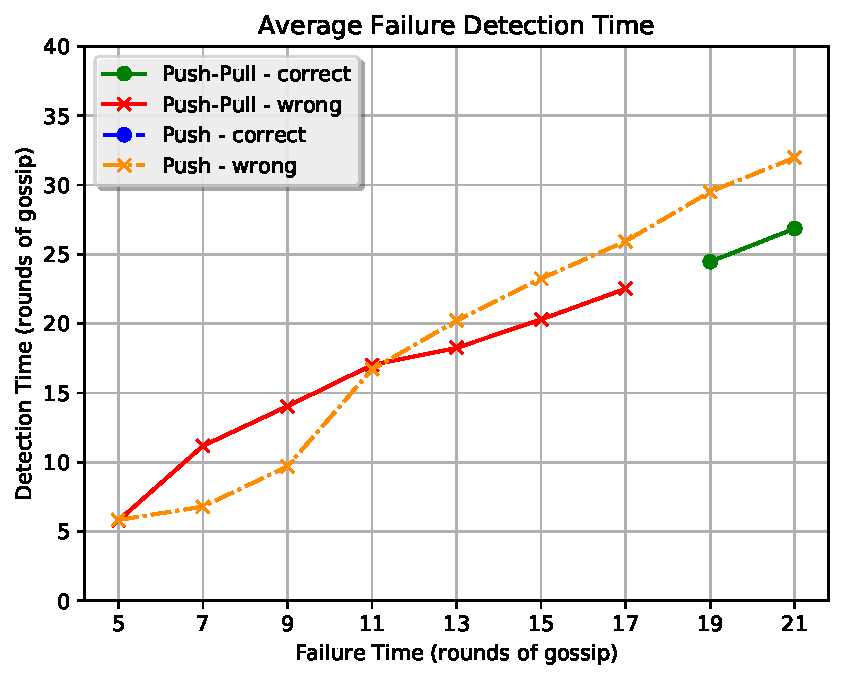
\includegraphics[width=\columnwidth]{figures/n50__average__s0__catastrophe__no_multicast}
	\caption{The plot shows the performances of the protocol in case of the sudden crash of $34$ of $50$ nodes. The multicast backup protocol in not enabled. Nodes choose their peers randomly (original strategy) and gossip every $200 \si{ms}$. The Push variant always fail to correctly report all and only the real crashes. The push-pull variant seems to work with high values of $T_{fail}$.}
	\label{fig:n50__average__s0__catastrophe__no_multicast}
\end{figure}

Some of the experiments are performed to understand how the failure detector behaves when the status of the system suddenly changes.
In particular, we try to understand if the failure detector keeps working correctly (it behaves as a perfect detector) even when \nicefrac{2}{3} of the nodes of the system crash simultaneously. 

As we expected, the failure detector is unable to report crashes correctly with reasonable $T_{fail}$ values.
In catastrophic scenarios, a node has not enough time to update its information about the status of the other nodes before the fixed timeout.
Survived nodes will push their information to crashed nodes wasting the message.
They will not be able to understand who survived the catastrophe before their respective fail timeouts are triggered, reporting also correct nodes as crashed.

\cref{fig:n50__average__s0__catastrophe__no_multicast} shows the Push-Pull strategy with high values of $T_{fail}$ detected crashed nodes without false positives. However, following repetitions of the experiment with the same and higher values of $T_{fail}$ shows that this is not always the case:
in most cases the failure detector does not work correctly despite the high $T_{fail}$.

\begin{figure}[t]
	\centering
	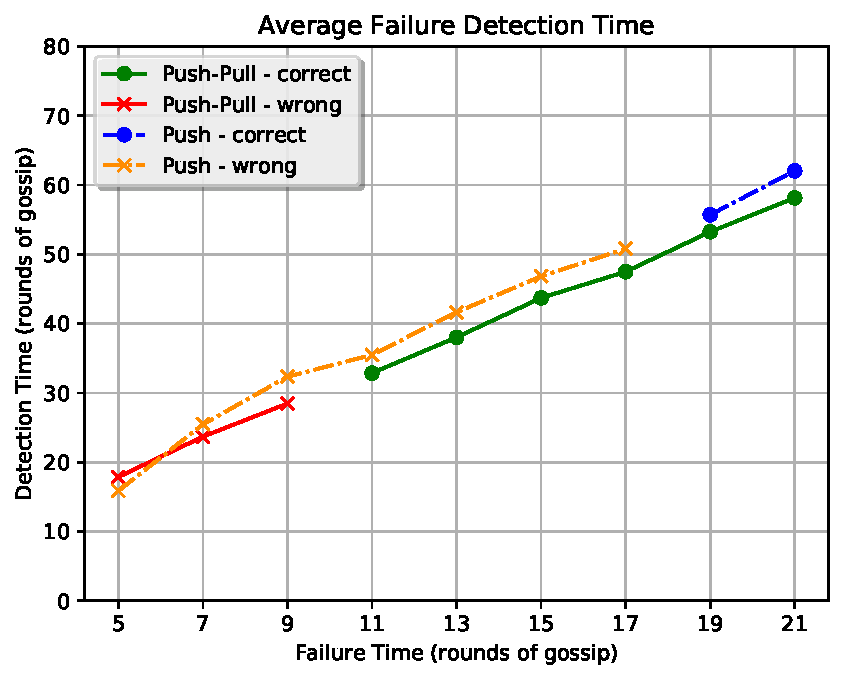
\includegraphics[width=\columnwidth]{figures/n50__average__s0__catastrophe__multicast}
	\caption{The plot shows the performances of the protocol using multicast in case of the sudden crash of $34$ of $50$ nodes. Nodes choose their peers randomly (original strategy) and gossip every $200 \si{ms}$. Thanks to the multicast, also the Push variant starts performing correct detections for high values of $T_{fail}$.}
	\label{fig:n50__average__s0__catastrophe__multicast}
\end{figure}

The strategies to select a node to gossip with described in \cref{sec:variants} are particularly detrimental for the failure detector in this case.
Since the strategies consist in picking the nodes not heard about for a long time with higher probabilities, a node will try to contact exactly the crashed ones. This exacerbates the problem of wasted messages.

To deal with this kind of situation, additional time is granted ($T_{miss}$) so that survived nodes have the chance to find each other.
To ensure that an updated version of heartbeat counters exists, the multicast protocol is used.
The performances are shown in \cref{fig:n50__average__s0__catastrophe__multicast}.
The multicast protocol allows a node to quickly collect information about survived ones after a catastrophe.
This also causes the reset of timers of correct nodes and avoids false positives.

Catastrophe recovery comes with a cost in terms of detection time.
From the comparison of \cref{fig:n50__average__s0__no_catastrophe__no_multicast} and \cref{fig:n50__average__s0__catastrophe__multicast} one notices that the time to detect correctly a fail node approximately doubles for the same $T_{fail}$.
This depends on the fact that the algorithm awaits $T_{miss}$ time after that $T_{fail}$ time is occurred before considering a node as failed. In the experiments proposed in the figures, a $T_{miss}$ equal to $T_{fail}$ has been used.
Due to the slow dissemination caused by the catastrophe, one can expect the average detection time in that case to be even more skewed towards high values.

One can set a $T_{fail}$ value based on the requirements of the system for correctness, balancing detection time and accuracy for specific needs, and the number of crashed nodes the system should tolerate without catastrophe recovery.
$T_{miss}$ is the next parameter to be defined.


\subsection*{Behaviour with respect to $T_{miss}$}

Since after a catastrophe the number of participating nodes decreases,
gossip messages will not take longer than $T_{fail}$ to spread with the same probability as before.
By setting $T_{miss} = T_{fail}$, the information obtained from the multicast protocol should have enough time to travel through all the remaining nodes.
However, we can make the case of the following problematic scenario. One node A is about to report another that is correct, when catastrophe happens. Theoretically, it may take too much time before gossips from the multicast protocol infects A. We argue that a mild catastrophe does not hinder normal functioning enough to result in that scenario, and on the other hand a more severe one would still require less than $T_{miss}$ to spread the information among surviving members.

\begin{figure}[t]
	\centering
	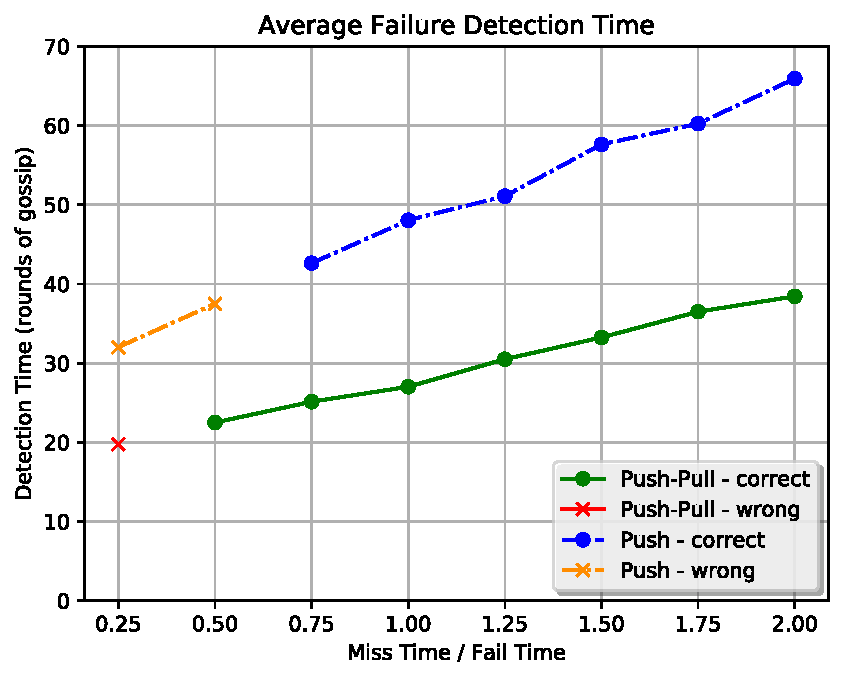
\includegraphics[width=\columnwidth]{figures/n50__miss_times}
	\caption{The plot shows the performances of the protocol using multicast in case of the sudden crash of $34$ of $50$ nodes for different $T_{miss}$. The experiment is performed with a $T_{fail}$ equals to $11$ rounds of gossip for the Push-Pull strategy and $19$ for the Push one. Nodes choose their peers randomly (original strategy) and gossip every $200 \si{ms}$.}
	\label{fig:n50__miss_times}
\end{figure}

Our experiments confirm this hypothesis.
\cref{fig:n50__miss_times} show the behaviour of the protocol in catastrophic conditions for a fixed $T_{fail}$ ($11$ rounds of gossip for the Push-Pull strategy and $19$ for the Push one).
For both strategy, $T_{miss} = T_{fail}$ gives a perfect failure detector.
$T_{miss} = 0.75 \cdot T_{fail}$ seems also to work in both cases, but does not provided a significant boost in the performances.
Since we want the algorithm to be very resilient even in catastrophic situations, we suggest to be slightly more conservative and simply use $T_{miss} = T_{fail}$.
The performances of the protocol can be tuned by changing $T_{fail}$ instead, depending on the real case scenario.


\subsection*{Push vs. Push-Pull}

As described at the beginning of this section, all the experiments are performed using the Push and Push-Pull gossip strategies with a fixed $T_{gossip}$ value of $200 \si{ms}$.
The failure detection algorithm that uses the Push-Pull approach performs always better than the algorithm that use Push.
Such a comparison in not completely fair.

With the Push strategy, each node receives an update on average one time in each round of gossip.
In particular, the expected number of updates can be computed as the probability to be chosen from a node multiplied by the number of nodes in the system.
Since the probability to pick a node has a uniform distribution, the expected number of updated for each node for each round of gossip is exactly one.

In the Push-Pull strategy, a node replies to the sender when it receives an update.
So, a node gets an update in 2 cases: every time it gossips with a not-crashed node and when it is chosen as a peer.
Since we assume independent crashes, we can approximate the probability to gossip with alive node to $1$.
This gives an expected number of updates for each round of gossip equals to roughly $2$.

% When the failure detector algorithm adopts the Push strategy, a node updates another one sending its list of nodes' heartbeats every $T_{gossip}$ (200 \si{ms} in our experiments) and receives information from another node with a probability of 1- Pmistake (?) as described in the paper.

% With the adoption of the Push-Pull strategy, a node that gossips has the opportunity to receive new information also from the node that it contacted (if it is not a crashed one) increasing the probability of the node of obtaining new information in a round of gossip. Therefore, when Push-Pull strategy is used, we can say that almost every $T_{gossip}$ time a node performs a Push and sends its information to other nodes two times: the first time when it contacts a random node with which gossip to and the second time when it replies to an incoming Push-Pull request from another node. 

To evaluate if the Push-Pull strategy really gives an advantage, we perform some experiments halving the $T_{gossip}$ time of the ``Push strategy'' experiments with respect to the $T_{gossip}$ time of the ``Push-Pull strategy'' ones.
We set a $T_{gossip}$ value of $200 \si{ms}$ for the experiments using Push and a $T_{gossip}$ of $400 \si{ms}$ for the experiments using Push-Pull.
The results reveals that the failure detection algorithm adopting the Push-Pull performs still better than the Push one even when its $T_{gossip}$ value is doubled.
A similar experiment with $T_{gossip} = 100 \si{ms}$ for Push and $T_{gossip} = 200 \si{ms}$ for Push-Pull yields the same results.
Comparison experiments have varying $T_{fail}$ (number of rounds corresponding to the same $T_{fail}$ differs between Push and Push-Pull since they have two different $T_{gossip}$). The Push-Pull variant remains correct with $11$ rounds, Push with $23$; Push-Pull obtains slightly lower average detection times as previously observed. Push-Pull can be used with node selection strategies (to obtain updates from quiescent members).

\subsection*{Node selection strategies}

If a node's timeout is approaching, it makes sense to contact it in a Push-Pull fashion to obtain its heartbeat counter. 
It comes out implementing a non-random choice does not allow for significantly lower $T_{fail}$ values. We did not observe improvements in that sense.
If the system can tolerate false positives favouring detection time, strategies seem to help to achieve greater accuracy.
In any case, the benefits of selection strategies were not substantial and not consistent (for consistency, longer experiments are required).
With 50 nodes, strategies did not make any significant impact on the performance.


\section{Conclusions}
\label{sec:conclusions}

In this work, we implemented a gossip-based protocol based on the paper ``A Gossip-Style Failure Detection Service'' of Van Renesse, Minsky and Hayden.
We tested and validated with multiple experiments in normal and extreme conditions the validity of the gossip approach to build a perfect failure detector.
We also proposed some variants to the protocol, such as different strategies for the peer selection and the Push-Pull approach for the gossip protocol.

The results of our experiments confirm the power of gossip protocols to solve difficult problems in an efficient way.
The Push-Pull strategy achieved better performances in all conditions.
Even though the analytical proof is very complex and out of the scope of this work, we strongly believe the Push-Pull strategy to outperform Push in almost every scenario.

In general, the alternative strategies proposed to select gossip recipients achieve performances comparable to the original one (pure random choice).
In the case of catastrophes, they are detrimental.
The randomness of the original strategy helps the protocol to better survive in extreme conditions.
Although is it probably possible to find out better strategies under very specific hypothesis, we believe it is not worth.
The random choice resulted to be very simple to implement, resilient and efficient.

The backup multicast algorithm is fundamental to recover from catastrophic scenarios such as the sudden and synchronized crash of \nicefrac{2}{3} of the nodes in the network.
This may be realistic in very extreme cases, but very unlikely in real world applications.
Depending on the specific scenario, one can choose to turn on or off the backup protocol.

The Internet has changed a lot from 1998, when the original work was published.
With the modern infrastructure, network capabilities and computing power, we do not need the level of optimization of resources consumptions needed in 1998.
This allows us to arbitrary tune the performances wanted from such a protocol depending on our needs.
In particular, a very simple way to do this is to change the gossip time.
Lower gossip times will produce a higher load on the infrastructure, but will achieve very fast failure detections.
Since the average failure detection time scales as \nobreak{$O(n\nobreak\hspace{.08em}\cdot\nobreak\hspace{.08em}log(n))$} with respect to the number of nodes, we can achieve very good results with a moderate consumption of network resources.



\bibliographystyle{IEEEtran}
\bibliography{references}

\end{document}
